\author{'Jakob Schlager'}

\section{Grundidee}
Bei der Entwicklung des Designs der Applikation wurde besonders darauf geachtet, eine benutzerfreundliche und gleichzeitig schlichte Benutzeroberfläche zu schaffen. Der Fokus lag darauf, die Anwendung so einfach wie möglich zu gestalten, ohne auf wichtige Funktionalitäten oder Flexibilität zu verzichten. Die Entscheidung, ein minimalistisches Design zu wählen, basiert auf der Überzeugung, dass eine cleane und aufgeräumte Oberfläche den Benutzer nicht überfordert, sondern ihm hilft, sich besser auf die wesentlichen Inhalte und Funktionen zu konzentrieren.

Ein zentraler Aspekt des Designprozesses war, den Entwicklern die Möglichkeit zu geben, den grundlegenden Aufbau der Anwendung festzulegen, während den Benutzern die Freiheit gewährt wird, das Layout nach ihren eigenen Bedürfnissen anzupassen. So können sie entscheiden, wie die Informationsboxen angeordnet sind, welche Primärfarbe für den Hintergrund verwendet wird und viele weitere Anpassungen vornehmen, um die Anwendung zu personalisieren. Dies fördert nicht nur die individuelle Nutzererfahrung, sondern unterstützt auch eine größere Anpassungsfähigkeit und Benutzerzentrierung, da verschiedene Nutzer unterschiedliche Bedürfnisse und Vorlieben haben.

Inspiriert von der minimalistischen und flexiblen Struktur von Applikationen wie \textbf{Notion}, wurde das Design mit dem Ziel entwickelt, eine hohe Anpassungsfähigkeit zu ermöglichen, während gleichzeitig eine klare und intuitiv verständliche Benutzeroberfläche erhalten bleibt. 


\begin{figure}[H]
    \centering
    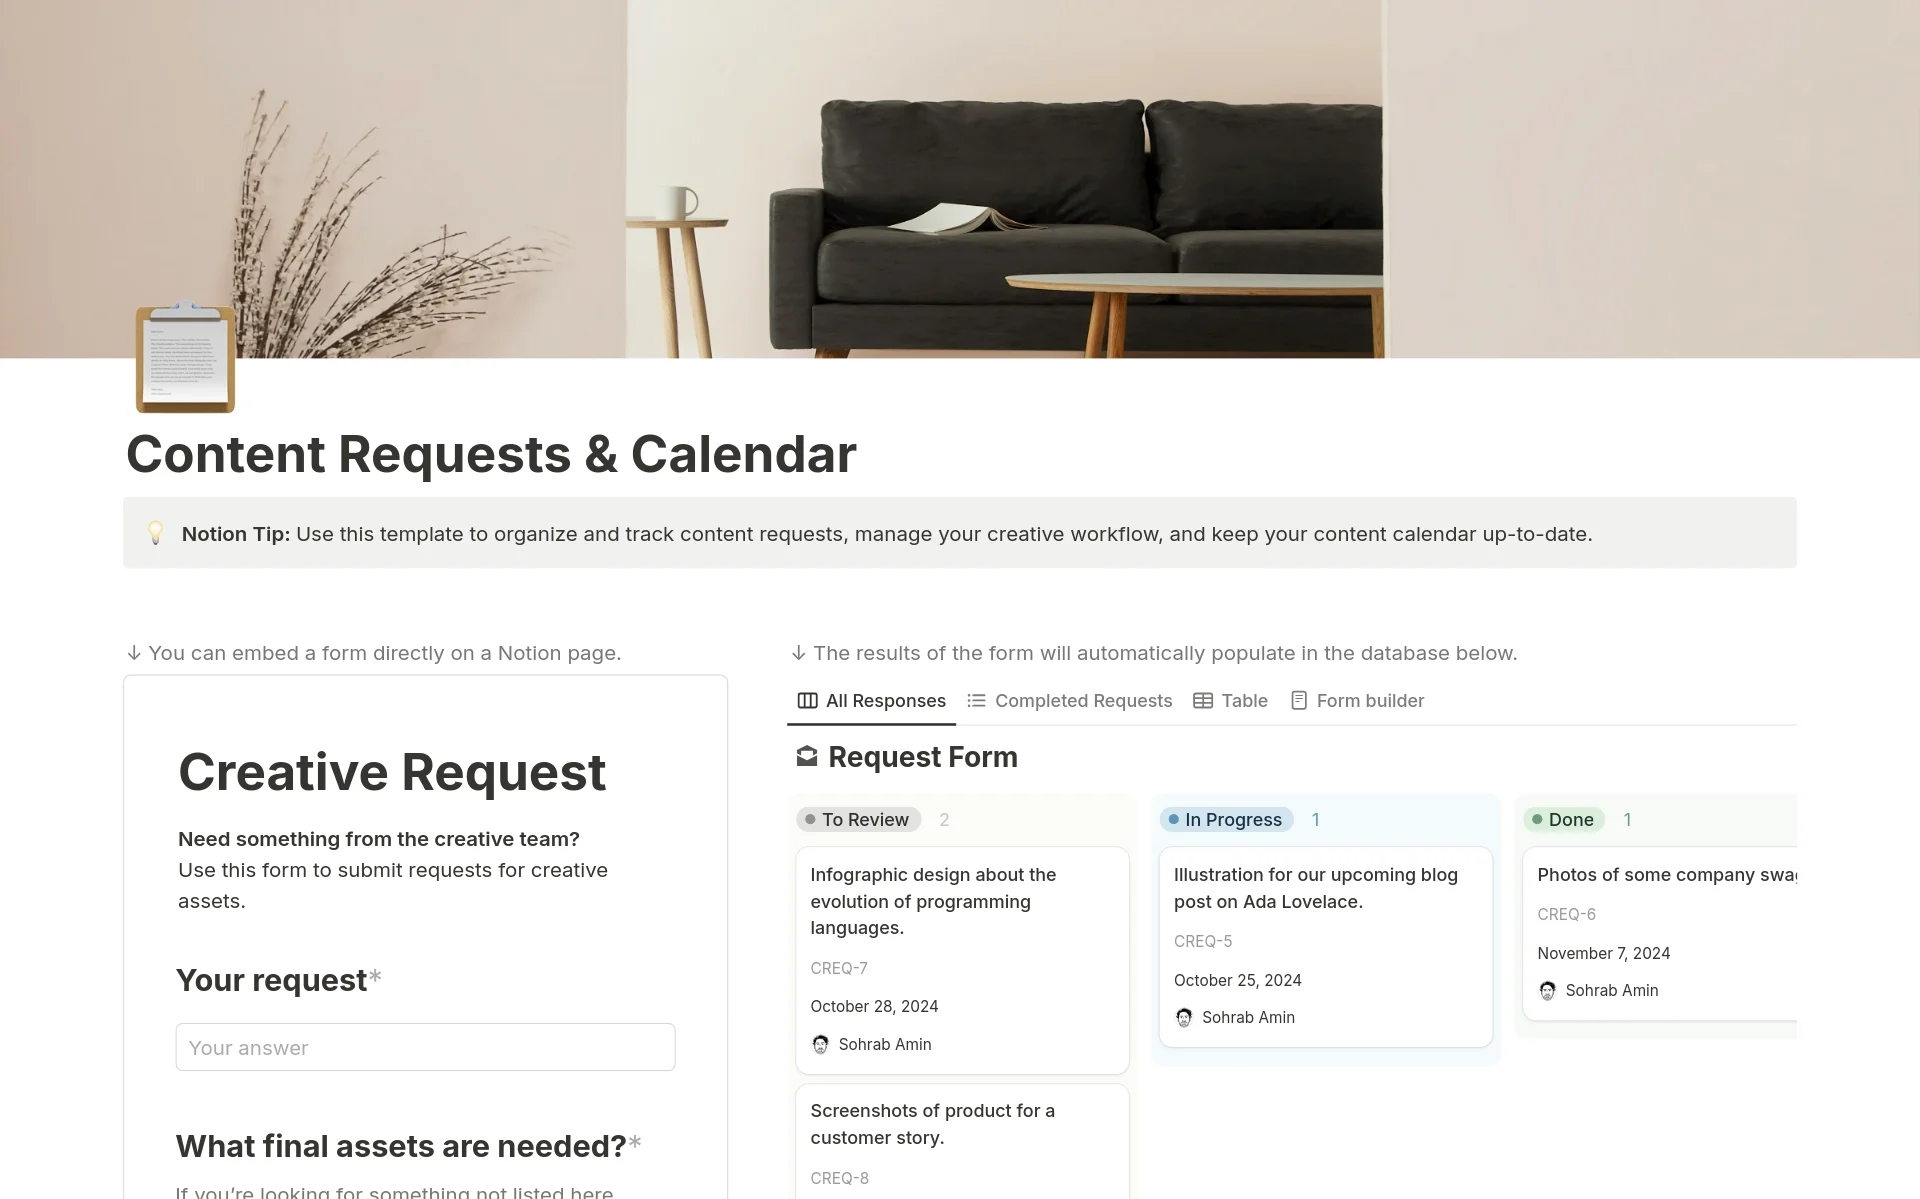
\includegraphics[scale=0.2]{pics/Design/NotionShowcase2.png}
    \caption{Abbildung des Notion Layouts}
    \label{fig:impl:notion}
\end{figure}

Ein weiterer Vorteil eines simplen Designs ist die Reduzierung von kognitiver Belastung. Durch die Wahl eines minimalistischen Ansatzes werden unnötige Elemente und Ablenkungen vermieden, was es dem Benutzer ermöglicht sich zuerst auf seine wirklich wichtigen Aufgaben zu konzentrieren, und anschließend sich mit dem Aussehen seiner Seite auseinanderzusetzen. Diese Kombination bietet eine hohe Benutzerbindung und fördert zudem die Zufriedenheit. Dies war ein entscheidender Punkt in der Designentwicklung, da man davon überzeugt war, dass eine klare und anpassbare Benutzeroberfläche langfristig zu einer besseren Nutzererfahrung führt und die Akzeptanz der Anwendung steigert.

Letztlich wurde beim Design der Applikation eine Balance zwischen Schlichtheit und Funktionalität angestrebt, bei der die Benutzeroberfläche nicht nur ästhetisch ansprechend, sondern auch funktional und benutzerfreundlich bleibt


\section{Das Logo und die ersten Entwürfe}
Das Logo stellt eines der zentralen Elemente der visuellen Identität einer Applikation, Firma, Unternehmens etc. dar. Auch bei \textbf{Melius} wurde eine intensive Auseinandersetzung mit der Frage vorgenommen, wie die mögliche Kreativität, die drei primären Farben sowie die Möglichkeit, alle wichtigen Dokumente und Informationen auf einer Website zusammenzufassen, in einem schönen und einfachen Logo adäquat reflektiert werden können.
Da ein Farbroller wichtig für die Arbeit eines Malers ist, wurde sich überlegt, diesen in Zusammensetzung mit dem Ordner als primäres Symbol für das Projekt zu wählen.

\subsection{Erster Entwurf}

\begin{figure}[H]
    \centering
    
\includegraphics[width=0.75\linewidth]{pics//Design/Logo_Vers1_macLookalike.png}
    \caption{Erster Entwurf des Melius Logo}
    \label{fig:logo_vers1}
\end{figure}

Der erste Entwurf des Logos ist bewusst schlicht gehalten und erinnert durch seine klare, geometrische Form sowie die ausgewogene Struktur an einen Datei-Ordner des Betriebssystems \textbf{macOS}. Diese Assoziation wurde bewusst gewählt, um dem Logo eine moderne, benutzerfreundliche und zugleich funktionale Ästhetik zu verleihen, die eine unmittelbare Wirkung auf den Nutzer hat.

Der Schwerpunkt der ersten Version lag auf der Basisstruktur des Logos sowie der grundlegenden Idee seiner zukünftigen Entwicklung. Das Ziel war die Kreation eines einfachen, aber aussagekräftigen Symbols, welches eine unmittelbare Wiedererkennung ermöglicht und gleichzeitig hinreichend Flexibilität bietet, um in späteren Versionen des Designs eine weitere Verfeinerung zu ermöglichen. Die erste Version war weniger auf Detailtreue bedacht, sondern vielmehr auf eine klare und minimalistische Darstellung der wesentlichen Designelemente, welche das visuelle Konzept des Logos in seiner Essenz widerspiegeln.

\subsection{Zweiter Entwurf}

\begin{figure}[H]
    \centering
    
\includegraphics[width=0.75\linewidth]{pics//Design/Logo_Vers2_primaryColors.png}
    \caption{Zwischenentwurf des Melius Logo}
    \label{fig:logo_vers2}
\end{figure}

Der zweite Entwurf des Logos weist im Vergleich zur ersten Version bereits signifikante Fortschritte auf. Während der erste Entwurf durch eine zurückgenommene Farbgebung sowie eine minimalistische Gestaltung geprägt war, wurden in dieser Version mehrere entscheidende Verbesserungen und Erweiterungen vorgenommen.

\subsubsection{Veränderungen und Verbesserungen}
Die Integration der Hauptfarben stellt eine wesentliche Veränderung dar.
In der vorliegenden Version wurden drei Hauptfarben eingeführt, welche sowohl das Logo lebendiger erscheinen lassen als auch als Fundament für die visuelle Identität der gesamten Applikation dienen. Die genannten Farben wurden zu einem späteren Zeitpunkt konsequent in der Gestaltung der Website sowie anderer Applikationen verwendet, wodurch eine stärkere Wiedererkennung und Einheitlichkeit des gesamten Brandings gewährleistet wird.

\subsubsection{Verwendung von Farbverläufen}
Im Vergleich zur ersten Version, die durch flache Farben dominiert wurde, weisen die Elemente des Logos in dieser Version sanfte Farbverläufe auf. Dies resultiert in einer modernen und dynamischen Ästhetik, welche die visuelle Tiefe verstärkt und das Design insgesamt ansprechender gestaltet.

\subsubsection{Das Farbschema}
Im ersten Entwurf wurden die Elemente des Logos, wie beispielsweise die Farbrolle, in dezenten, einheitlichen Blautönen gehalten. In der zweiten Version hingegen wurden kontrastierende Farben verwendet. So wurde die Farbrolle beispielsweise in einem kräftigen Weiß oder mit einem Farbverlauf hervorgehoben, was sie optisch in den Vordergrund rückt und die Möglichkeiten für Kreativität und Anpassbarkeit der Anwendung besser vermitteln soll.

\subsection{Finaler Entwurf}

\begin{figure}[H]
    \centering
    
\includegraphics[width=0.75\linewidth]{pics//Design/Logo_Final_justPerfect.png}
    \caption{Finaler Entwurf des Melius Logo}
    \label{fig:logo_final}
\end{figure}

Wie man hier sehr gut erkennen kann, hat das Logo in der endgültigen Version im Vergleich zu den vorherigen Visualisierungen seine endgültige Form angenommen und wirkt nun deutlich ausgereifter. Der Schwerpunkt liegt auf der Harmonie zwischen den Elementen, der Modernität des Designs und der Klarheit der Symbolik.

Der einzige Unterschied zwischen den beiden Abbildungen des endgültigen Entwurfs, der nur schwer zu erkennen ist, besteht in der Sättigung der Farbstreifen unter dem Farbroller. Diese kleine, aber entscheidende Anpassung war Gegenstand einer ausführlichen Diskussion innerhalb der Schulkasse, ergänzt durch Rückmeldungen von verschiedenen Lehrer:innen. Nach einer gemeinsamen Abstimmung entschied man sich schließlich für die \textbf{rechte Version} des Logos.

Das endgültige Logo hebt die kreative Idee hinter dem Farbroller besonders hervor. Der Farbroller wurde so integriert, dass er nicht nur den Ordner zu „rollen“ scheint, sondern auch eine Verbindung zwischen Kreativität und Organisation schafft. Diese Darstellung soll symbolisieren, dass die im Ordner enthaltenen Informationen durch den Farbroller nicht nur zugänglich gemacht, sondern auch mit einer kreativen Note angereichert werden. Dadurch wird eine visuelle Verbindung zwischen der praktischen Funktionalität und der kreativen Inspiration des Projekts geschaffen.

Besonders hervorzuheben ist, dass die klaren Linien und die ausgewogene Farbgestaltung dem Logo eine professionelle und moderne Ästhetik verleihen. Die subtilen Farbübergänge im Ordner und die akzentuierte Darstellung des Farbrollers erzeugen eine dynamische Wirkung, die den Kerngedanken des Projektes optimal transportiert. Das Ergebnis ist ein Logo, das nicht nur funktional und ästhetisch ansprechend ist, sondern auch die Kernbotschaften des Projekts - Kreativität, Struktur und Innovation - perfekt visualisiert.


\section{Entwürfe der Website}

\subsection{Die Landing page}
Die Landing page der Anwendung Melius wurde mit dem Ziel entwickelt, den Benutzer bereits beim ersten Eindruck durch ein klares und ansprechendes Design zu überzeugen. Dabei wurden bewusste Entscheidungen getroffen, um sowohl die Kreativität als auch die Datensicherheit - zwei zentrale Werte der Anwendung - zu verdeutlichen.

\subsubsection{Design und Struktur}
Die Gestaltung der Landing page folgt einem minimalistischen Ansatz, um den Nutzer nicht zu überfordern und den Fokus auf das Wesentliche zu lenken. Die Seite ist zweigeteilt: Auf der linken Seite befindet sich in zentraler Position der Name der Anwendung „Melius“. Der Name ist in einer Kombination aus drei Primärfarben gehalten, was ihn nicht nur hervorhebt, sondern auch die Markenidentität stärkt. Direkt darunter befinden sich zwei Call-to-Actions (CTAs): Der blaue „Get Started“-Button, der als primärer CTA den Nutzer zur Registrierung motiviert und der dezentere „Login“-Button, der für bereits registrierte Nutzer gedacht ist.

Die rechte Seite der Landingpage wird vom zentralen Logo dominiert. Es zeigt einen Aktenordner in Kombination mit einer Farbrolle - ein starkes Symbol für Ordnung und Individualisierung. Der Hintergrund wird durch subtile, leicht transparente blaue Radiowellen ergänzt, die dem Design Dynamik und Tiefe verleihen, ohne vom Hauptinhalt abzulenken.

\subsubsection{Das Logo als zentrales Element}
Das Logo wurde bewusst als zentrales Element in den Vordergrund gerückt, da es die Kernfunktionen der Anwendung symbolisiert: die individuelle Anpassung und die sichere Verwaltung von Daten. Um die Vielseitigkeit und Kreativität von Melius zu unterstreichen, wurden mehrere Varianten für die Startseite entwickelt:


\subsubsection{Variation 1: Minimalistisch und Schlicht}
\begin{figure}[H]
    \centering
    
\includegraphics[width=0.75\linewidth]{pics//Design/Website/LandingPage/LandingPage_vers1.png}
    \caption{Erster Entwurf der Landing Page}
    \label{fig:lp_vers1}
\end{figure}
In der ersten Version präsentiert sich das Logo in einer reduzierten Form, ohne visuelle Elemente, was einen aufgeräumten und klaren Eindruck vermittelt.


\subsubsection{Variation 2: Integration kreativer Elemente}
\begin{figure}[H]
    \centering
    
\includegraphics[width=0.75\linewidth]{pics//Design/Website/LandingPage/LandingPage_vers2.png}
    \caption{Zweiter Entwurf der Landing Page}
    \label{fig:LandingPage}
\end{figure}
In der zweiten Version werden Icons und Symbole – darunter ein Haus, ein Upload-Icon und ein Personen-Symbol – in das Design integriert, die symbolisch für die vielfältigen Funktionen stehen. Die Datenpunkte, die aus der Mappe herauszuströmen scheinen, verdeutlichen die Offenheit und Interaktivität der Applikation.

\subsubsection{Variation 3: Finalisierte, strukturierte Darstellung}
\begin{figure}[H]
    \centering
    
\includegraphics[width=0.75\linewidth]{pics//Design/Website/LandingPage/LandingPage_versFinal.png}
    \caption{Finaler Entwurf der Landing Page}
    \label{fig:lp_vers1}
\end{figure}
In der finalen Version wurde das Konzept verfeinert, indem die Symbole und Datenpunkte sich radial um das Logo verteilen, wodurch die Struktur und Ordnung stärker hervorgehoben werden.
Die kreative Freiheit und die Sicherheit der Nutzer bei der Nutzung der Applikation werden durch die aus der Mappe hervorgehenden Symbole und Datenpunkte veranschaulicht. Die zahlreichen Möglichkeiten der individuellen Gestaltung von Profilen und der Visualisierung von Daten werden durch die Symbole und Datenpunkte verdeutlicht. Gleichzeitig signalisiert die klare und konsistente Farbgebung Vertrauen und Stabilität.


\subsection{Anmeldung und Registrierung}
Es lassen sich gemeinsame Designelemente feststellen.
Sowohl die Anmelde- als auch die Registrierungsseite basieren auf einem zweispaltigen Layout, das eine klare Aufteilung zwischen der Informations- und Navigationsseite (links) und der interaktiven Formularseite (rechts) bietet.
Die linke Seite enthält den Titel "Melius" und den Slogan "The Better Profile", die den zentralen Markenwert kommunizieren.Diese statischen Elemente bieten Orientierung und schaffen eine visuelle Verbindung zur allgemeinen Markenidentität, wie sie bereits auf der Landing Page etabliert wurde.

\subsubsection{Die Anmeldeseite}
\begin{figure}[H]
    \centering
    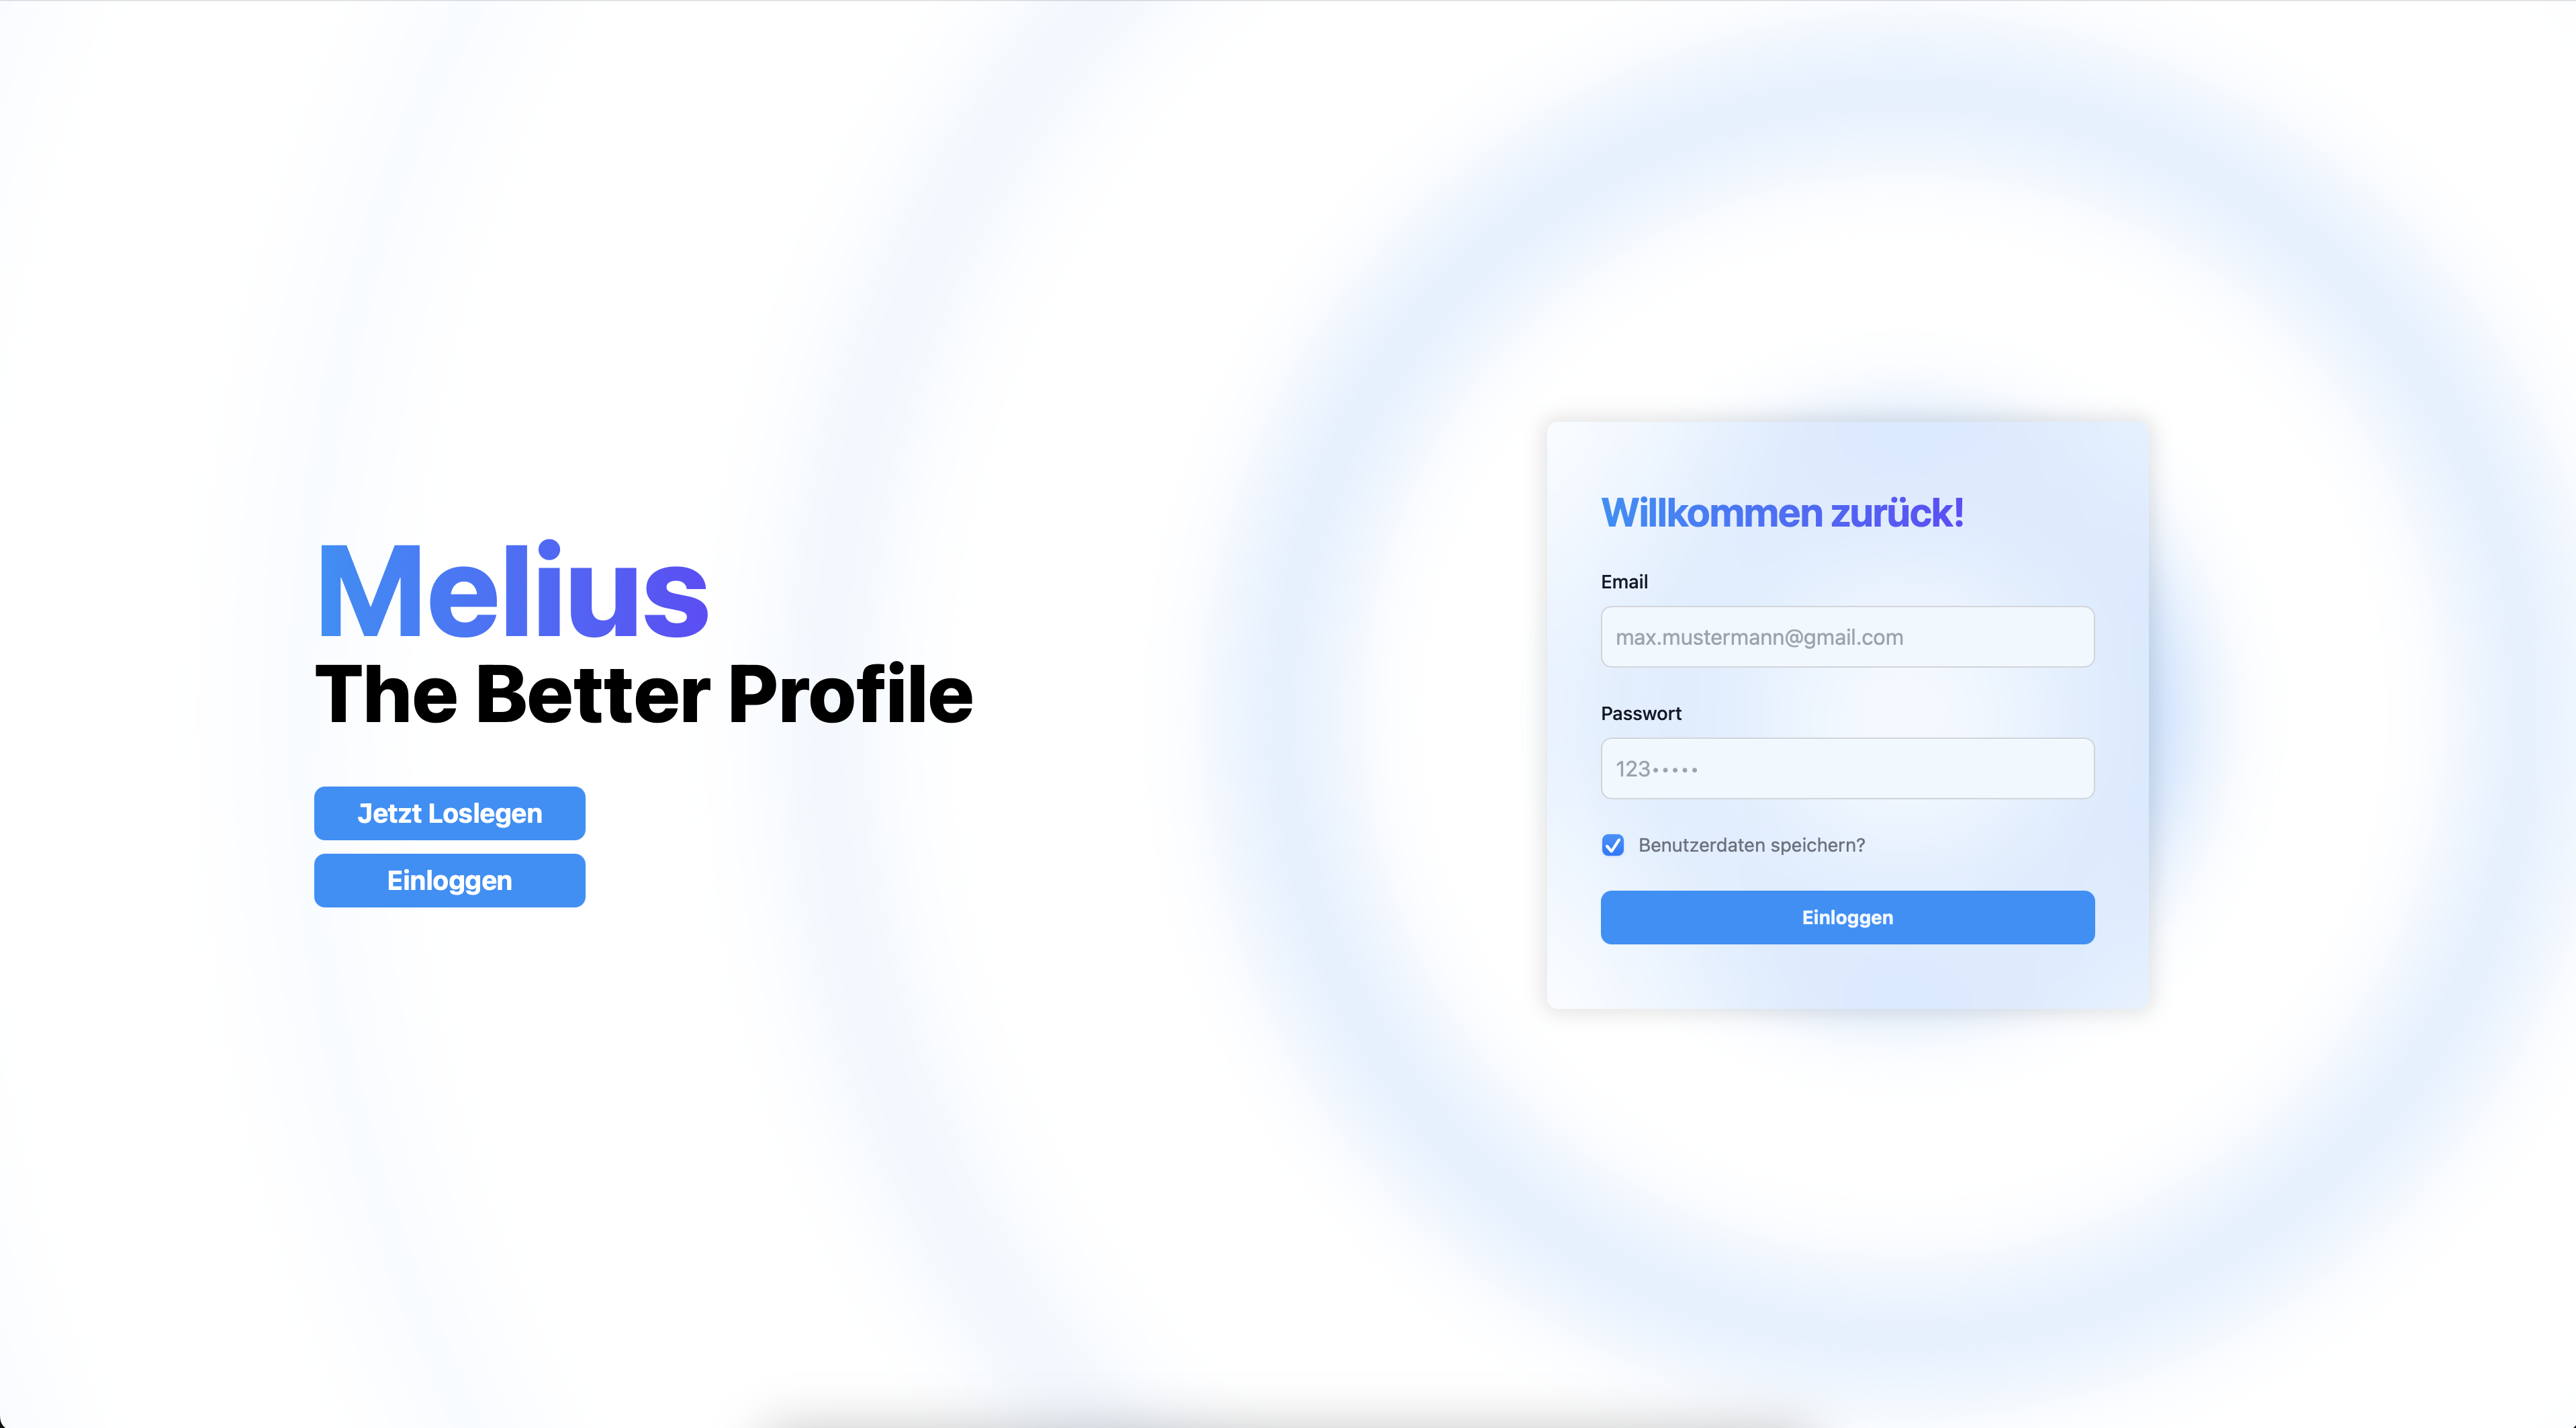
\includegraphics[width=0.75\linewidth]{pics//Design/Website/LandingPage/lp_Anmeldung.png}
    \caption{Anmeldeformular}
    \label{fig:Anmeldung}
\end{figure}
Die Anmeldeseite wurde speziell für bestehende Benutzer konzipiert und zeichnet sich durch ein schlankes und effizientes Design aus, wobei der Fokus auf der schnellen und einfachen Ermöglichung des Zugangs zu dem Benutzerkonto liegt.
Das Formulardesign ist auf Effizienz ausgelegt, wobei die Felder für E-Mail-Adresse und Passwort zentral und übersichtlich angeordnet sind. Beide Felder sind großzügig dimensioniert, um eine angenehme Eingabeerfahrung zu gewährleisten, und es stehen klare Platzhaltertexte zur Orientierung zur Verfügung.
    \begin{itemize}
        \item Das Formular umfasst die Felder E-Mail und Passwort, die zentral und übersichtlich platziert sind.Beide Felder sind ausreichend groß gestaltet, um die Eingabe komfortabel zu machen, und bieten klare Platzhaltertexte zur Orientierung.
    \end{itemize}
    \begin{itemize}
        \item Eine zusätzliche Checkbox mit der Beschriftung "Benutzerdaten speichern?" bietet den Benutzern die Möglichkeit, ihre Anmeldedaten für zukünftige Sitzungen zu speichern, was die Benutzerfreundlichkeit insbesondere für wiederkehrende Benutzer erhöht.
    \end{itemize}
    \begin{itemize}
        \item Der Button "Einloggen" ist in einem kräftigen Blauton gestaltet, um Aufmerksamkeit zu erzeugen und den nächsten Schritt klar zu kommunizieren.
    \end{itemize}
Darüber hinaus trägt die visuelle Abgrenzung dazu bei, dass die einzelnen Elemente auf dem Formular klar voneinander getrennt sind.
    \begin{itemize}
        \item Das Formular ist durch einen leicht transparenten und verschwommenen Hintergrund optisch hervorgehoben, ohne aufdringlich zu wirken, was es dem Benutzer erleichtert, sich auf die wesentlichen Elemente zu konzentrieren.
    \end{itemize}


\subsubsection{Die Registrierungsseite}
\begin{figure}[H]
    \centering
    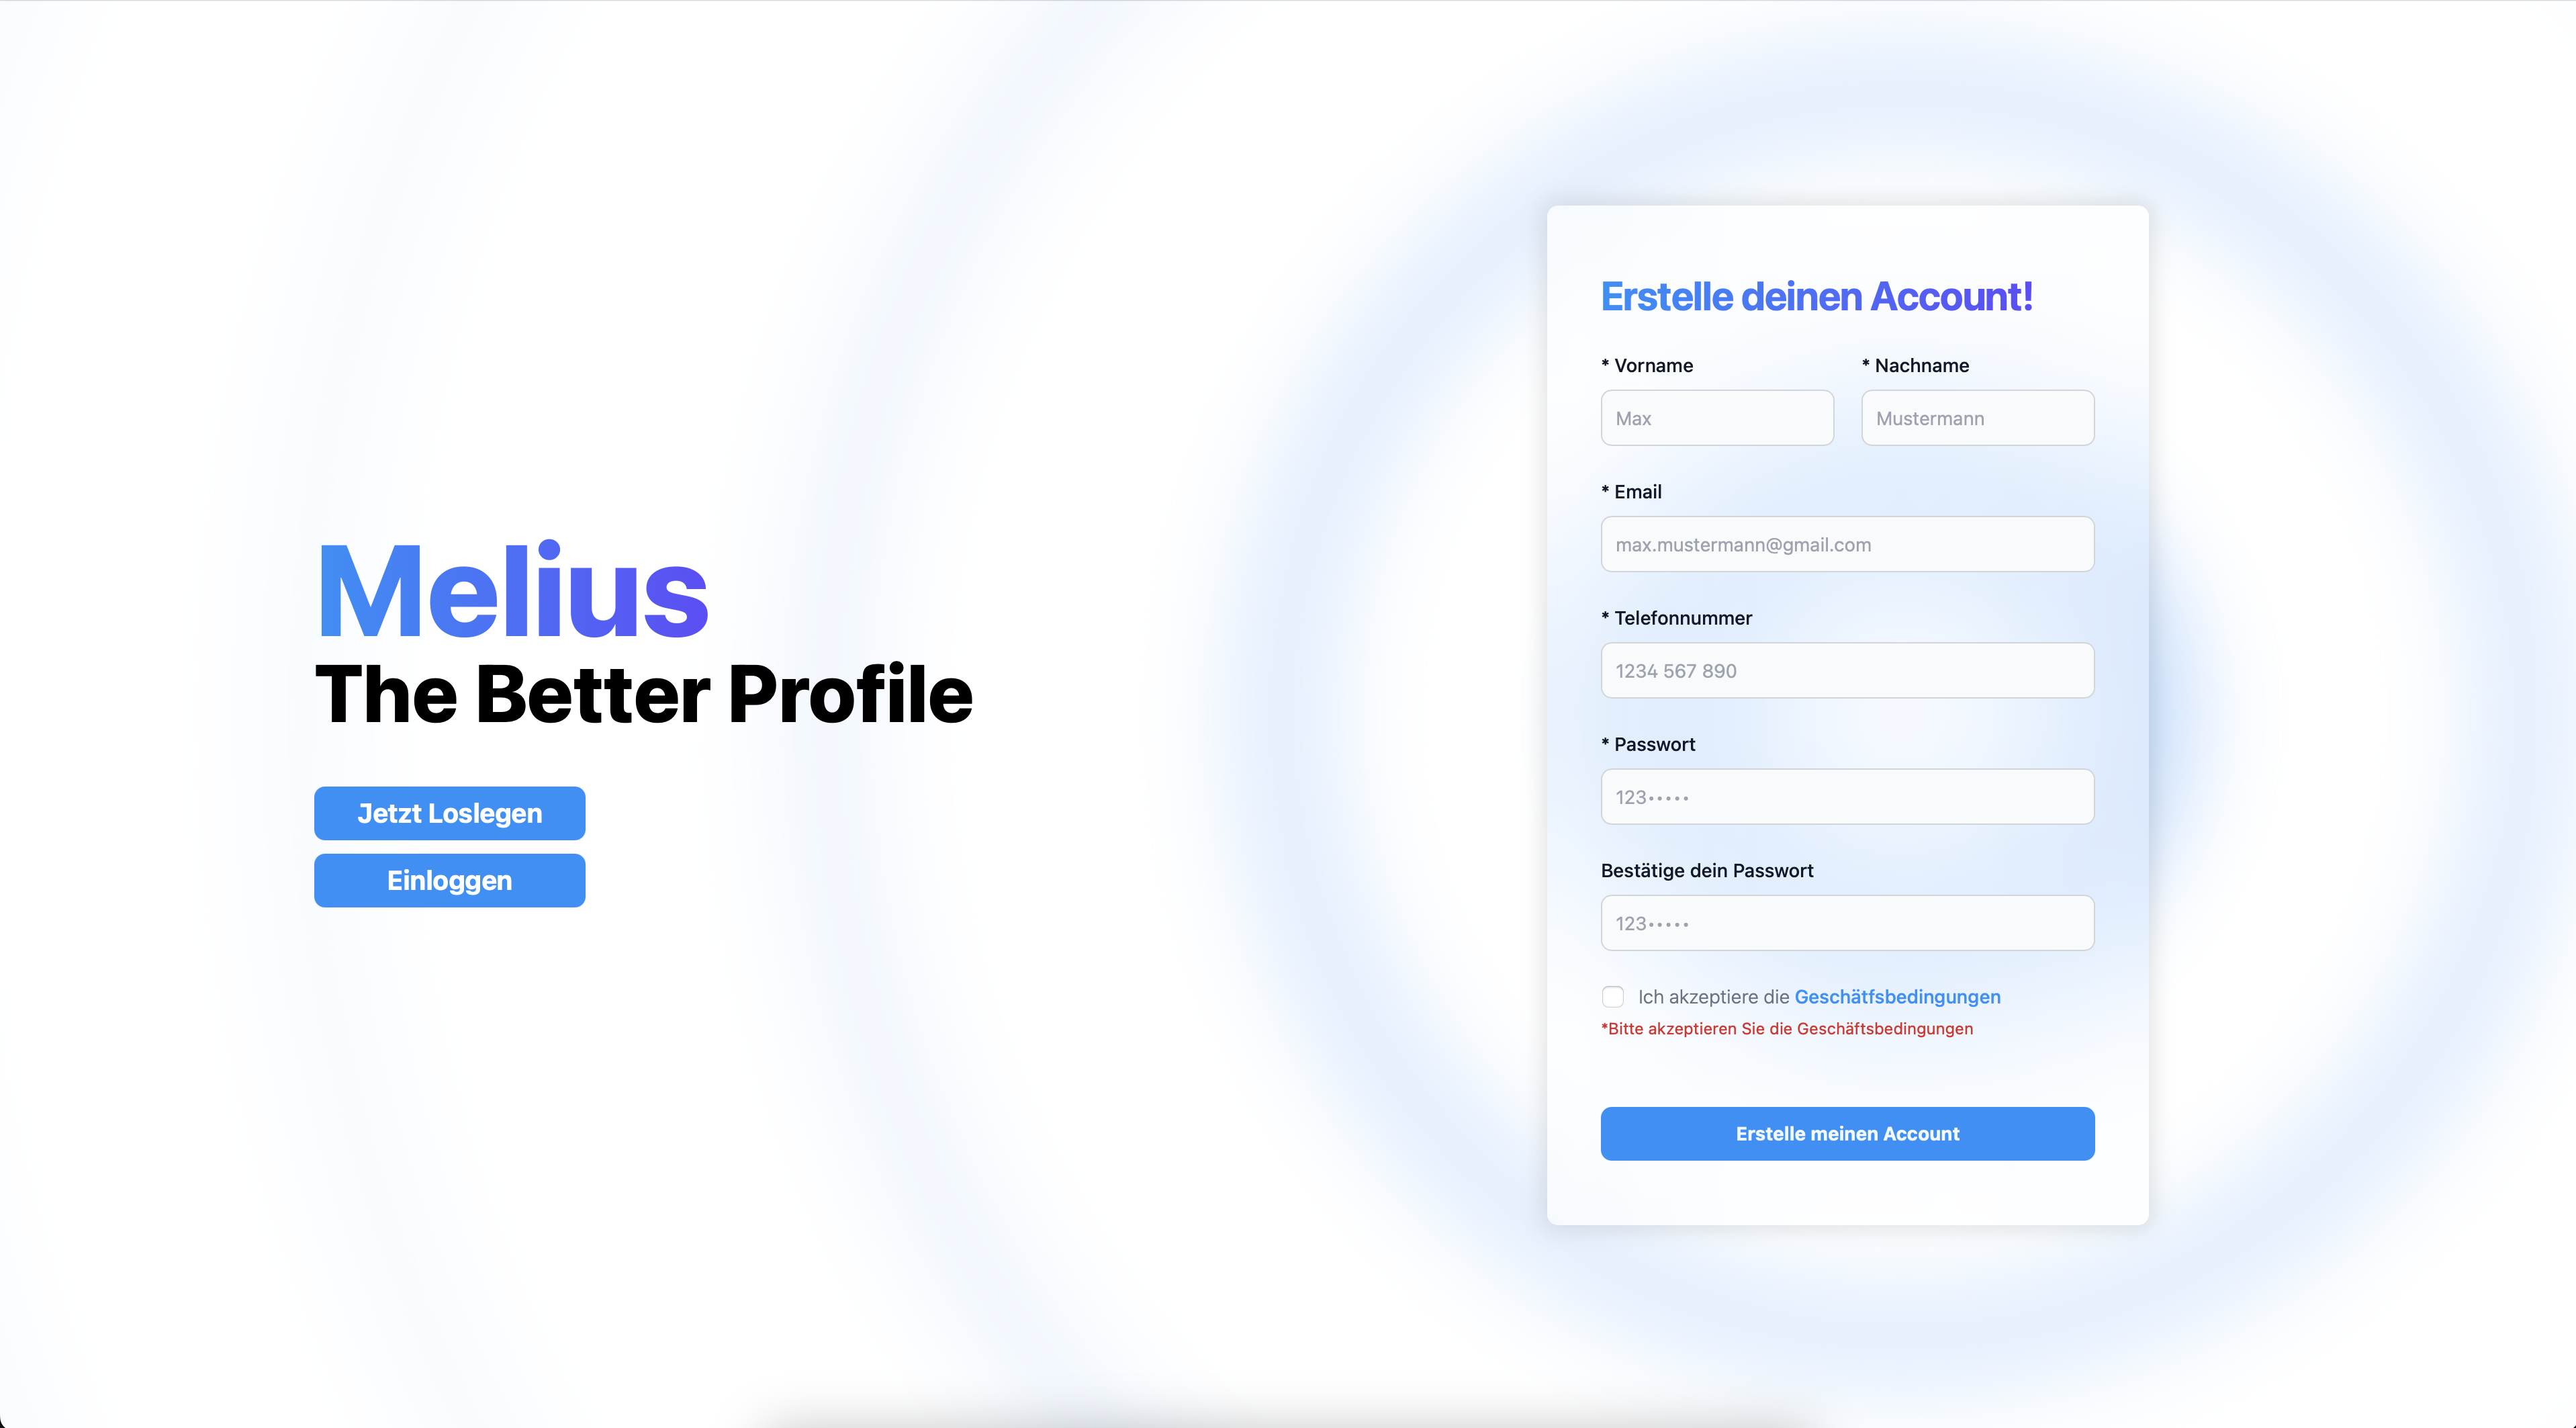
\includegraphics[width=0.75\linewidth]{pics//Design/Website/LandingPage/lp_Registrierung.png}
    \caption{Registrierungsformular}
    \label{fig:Registrierung}
\end{figure}
Die Registrierungsseite ist für neue Benutzer konzipiert, die ein Konto erstellen möchten. Da dieser Prozess eine höhere Anzahl an Informationen erfordert, ist das Formular umfangreicher gestaltet, ohne dabei an Klarheit zu verlieren.
Das Formulardesign ist darauf ausgerichtet, den Prozess der Kontoerstellung für neue Benutzer zu vereinfachen und zu beschleunigen.
\textbf{Das Formular enthält die folgenden Eingabefelder:}
        \begin{itemize}
            \item Vorname und Nachname: Zur Eingabe der persönlichen Daten.
        \end{itemize}
        \begin{itemize}
            \item E-Mail: Für die Registrierung der Kontaktadresse.
        \end{itemize}
        \begin{itemize}
            \item Des Weiteren besteht die Option, ein zusätzliches Kontaktfeld für Telefonnummern anzulegen, um die Kontaktmöglichkeiten zu erweitern.
        \end{itemize}
        \begin{itemize}
            \item Des Weiteren sind ein Passwort und dessen Bestätigung zur Erstellung eines sicheren Kontos erforderlich.
        \end{itemize}
    \begin{itemize}
        \item Am Ende des Formulars befindet sich eine Checkbox, mit der der Benutzer die Geschäftsbedingungen akzeptieren muss. Diese ist klar gekennzeichnet, und es wird eine Fehlermeldung angezeigt, wenn sie nicht angeklickt wurde.
    \end{itemize}
    \begin{itemize}
        \item Der Button "Erstelle meinen Account" ist in einem kräftigen Blau gehalten und leitet den Benutzer zum Abschluss der Registrierung.
    \end{itemize}
Das Formular ist durch eine logische Reihenfolge der Eingabefelder und deutliche Platzhaltertexte leicht verständlich.Die visuelle Abgrenzung durch den leicht transparenten und verschwommenen Hintergrund hilft, das Formular klar hervorzuheben.

\subsection{Die Startseite}
Das Design der Startseite folgt einem zeitgemäßen, schlichten und nutzerfreundlichen Konzept, das durch klare Strukturen und intuitive Navigation besticht.Die Gestaltung zielt darauf ab, dem Benutzer einen einfachen Einstieg in die verschiedenen Inhalte der Plattform zu ermöglichen, während es gleichzeitig eine ästhetische und professionelle Atmosphäre schafft.

\begin{figure}[H]
    \centering
    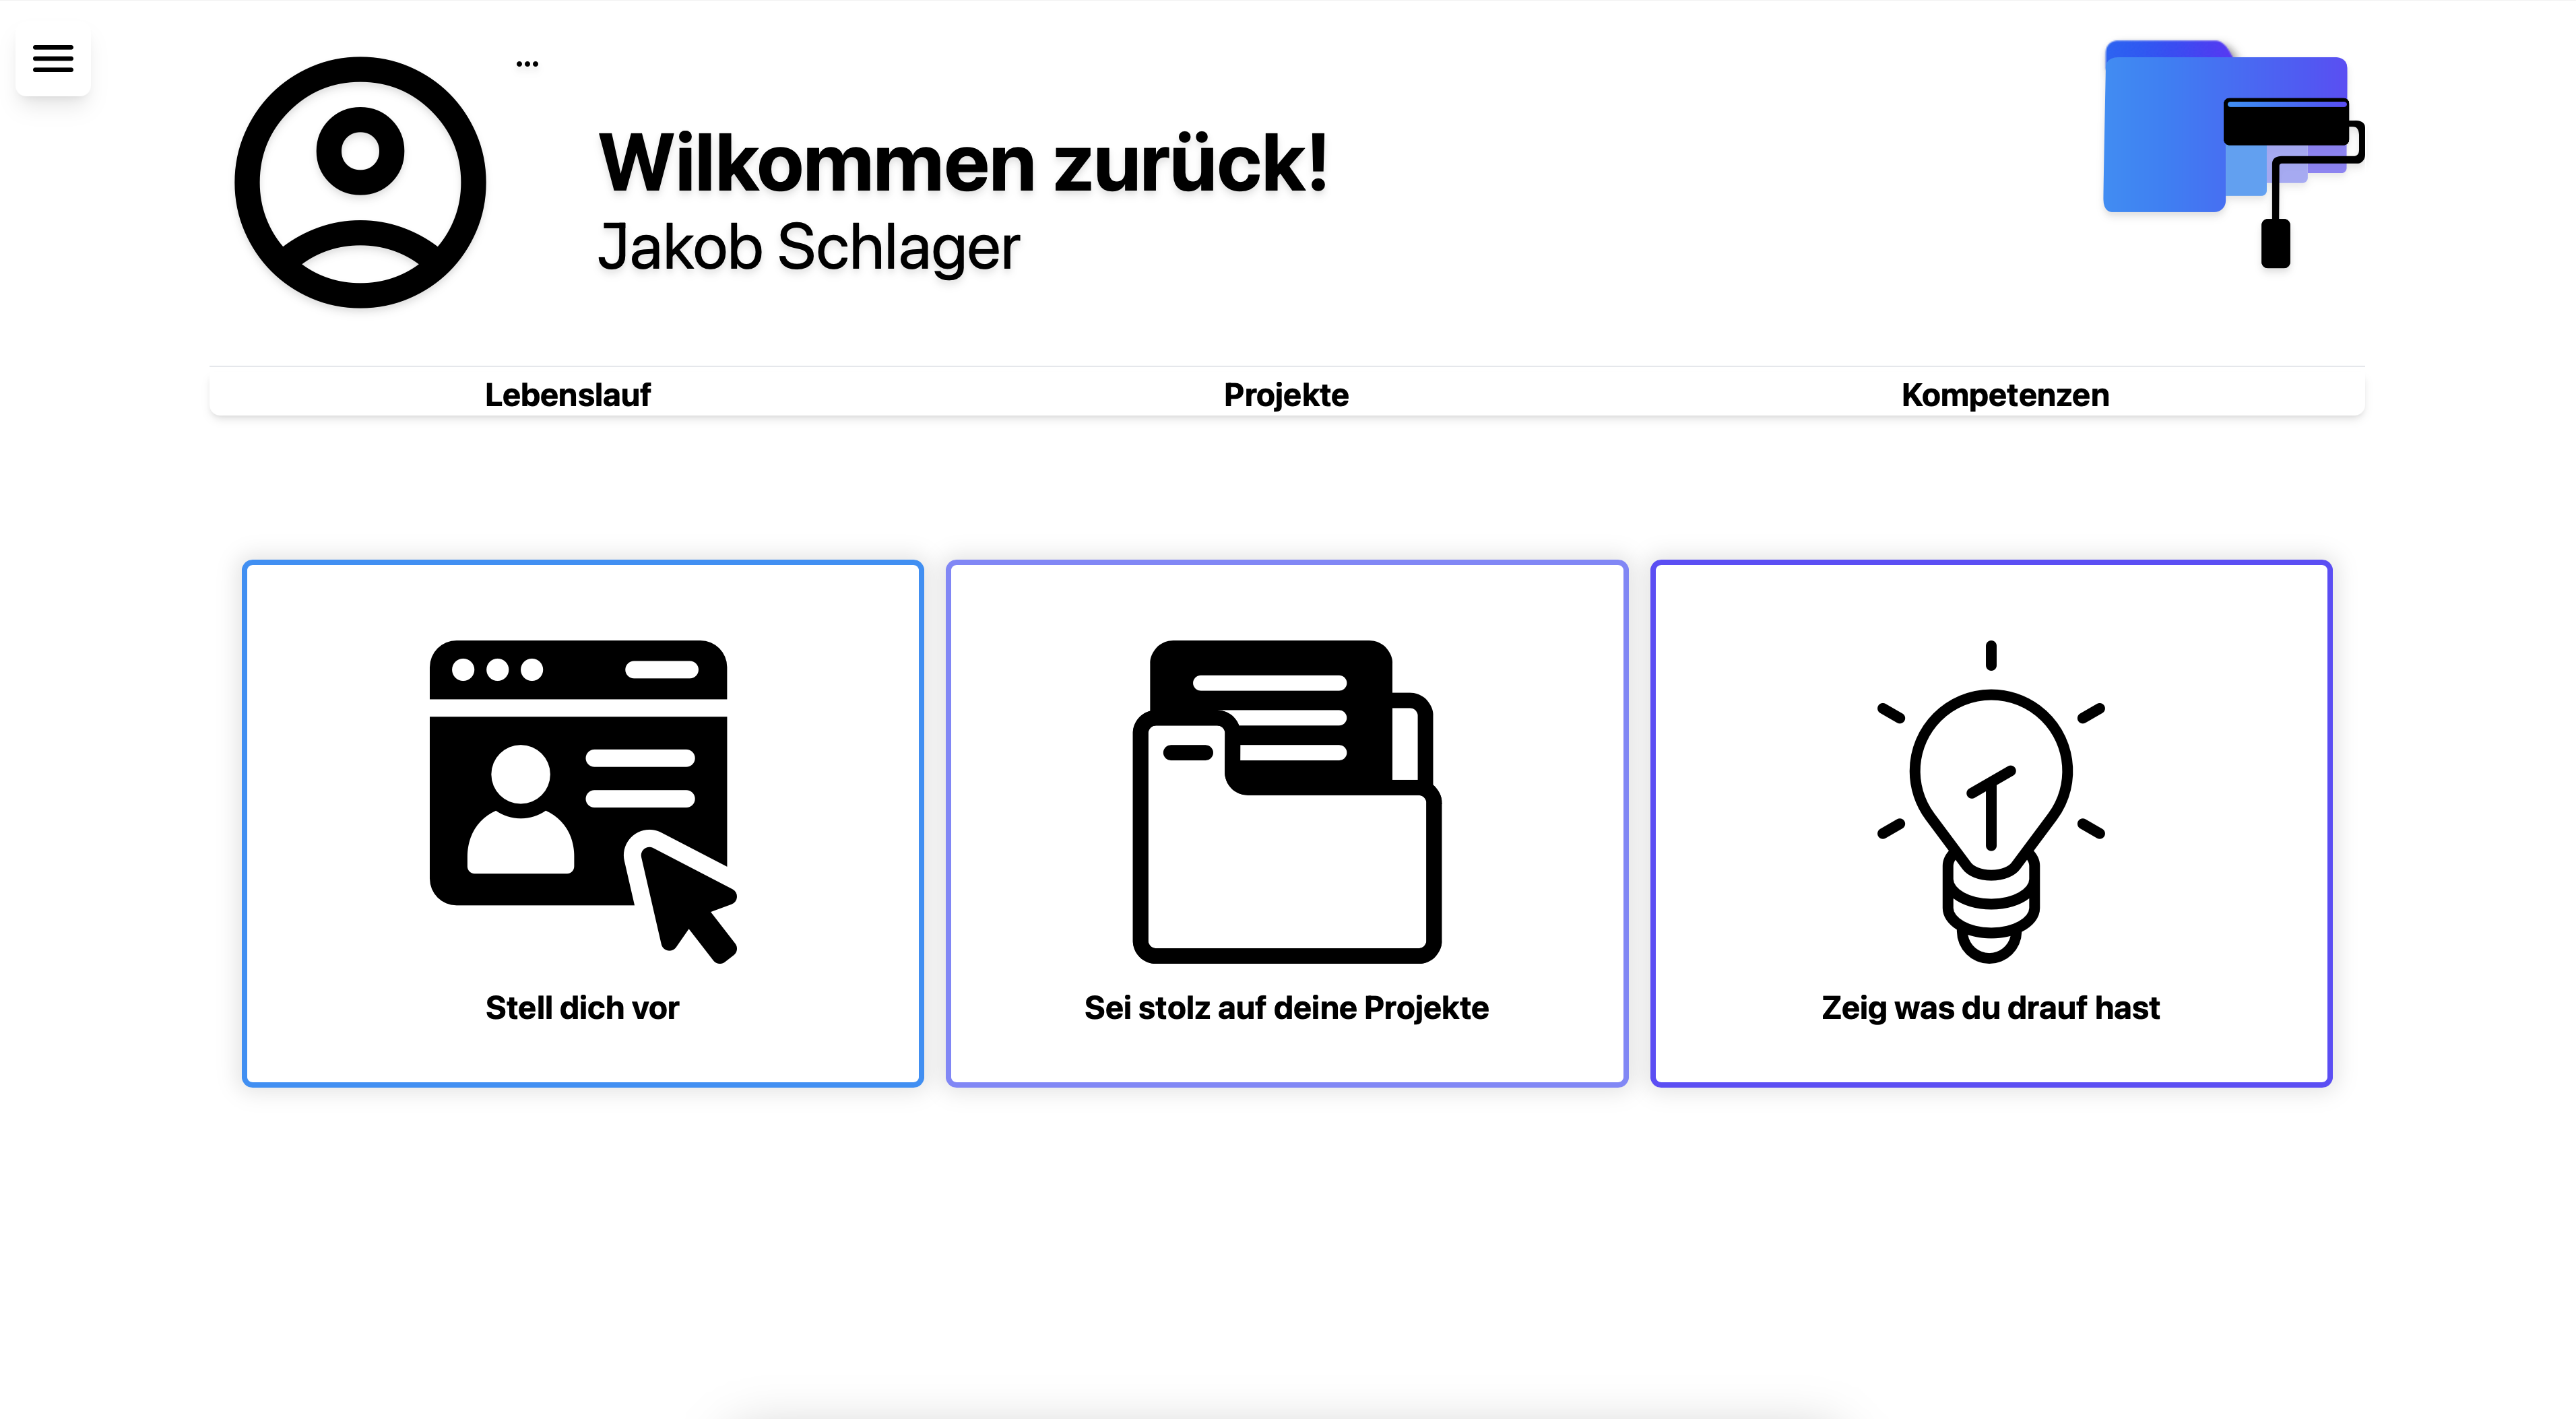
\includegraphics[width=0.75\linewidth]{pics//Design/Website/Startseite/Startseite.png}
    \caption{Startseite}
    \label{fig:Startseite}
\end{figure}

\subsubsection{Der Willkommens-Bereich}

Die Kopfzeile der Startseite präsentiert die Benutzerinformationen und zentralen Funktionen in einer klaren und übersichtlichen Form. Im linken Bereich wird ein großes, kreisförmiges Standard-Profilbild angezeigt, unmittelbar gefolgt von einer personalisierten Begrüßung mit dem Namen des Benutzers, was eine maßgeschneiderte Benutzererfahrung gewährleistet.Ein zentrales Element ist das Dropdown-Menü, das durch ein kleines Dreipunkt-Symbol aufgerufen werden kann. Dieses Menü bietet zwei Optionen:

\begin{itemize}
    \item "Profilbild hinzufügen": Der Benutzer kann ein eigenes Bild hochladen.
\end{itemize}

\begin{itemize}
    \item "Profilbild entfernen": Falls bereits ein Bild gesetzt wurde, kann es wieder entfernt werden.
\end{itemize}
Auf der rechten Seite des Headers befindet sich das Melius-Logo, das aus einer blauen, stilisierten Akte mit einer schwarzen Farbrolle besteht.Dieses visuelle Element unterstreicht das Corporate Design der Plattform und sorgt für einen professionellen Wiedererkennungswert.

Die Kopfzeile vereint somit eine klare Benutzerführung mit einer personalisierten Gestaltung und bietet dem Benutzer eine intuitive Möglichkeit, sein Profil anzupassen.

\begin{figure}[H]
    \centering
    
\includegraphics[width=0.75\linewidth]{pics//Design/Website/Startseite/Header.png}
    \caption{Kopfzeile}
    \label{fig:Kopfzeile}
\end{figure}


\subsubsection{Die interaktiven Boxen}
Der Fokus liegt auf den drei großen, visuell ansprechend gestalteten, interaktiven Kacheln im Zentrum der Seite, die gleichzeitig als zusätzliche Navigation dienen. Sie repräsentieren die Unterseiten "Allgemein", "Projekte" und "Kompetenzen".
\begin{itemize}
    \item Die linke Box, die den Titel "Stell dich vor (Lebenslauf)" trägt, ermutigt den Benutzer, persönliche Informationen zu hinterlegen oder sich vorzustellen. Das Icon eines Profilbilds auf einer Webseite symbolisiert diesen Bereich perfekt.
\end{itemize}
\begin{itemize}
    \item Die Präsentation der eigenen Projekte (Projekte) wird in der mittleren Box angeregt. Die Darstellung einer Mappe mit Dokumenten verdeutlicht die Funktionalität, eigene Arbeiten zu strukturieren und sichtbar zu machen.
\end{itemize}
\begin{itemize}
    \item Die rechte Box, die mit einer Glühbirne versehen ist, steht für Kreativität und Kompetenzen und lädt dazu ein, eigene Kompetenzen und Stärken zu präsentieren und hervorzuheben.
\end{itemize}
Die Abgrenzung der einzelnen Boxen sowie die Verwendung von Primärfarben tragen zur optischen Anmutung bei und ziehen die Aufmerksamkeit der Benutzer:innen auf sich. Die reduzierte Farbpalette in Kombination mit den minimalistischen Icons erzeugt eine aufgeräumte und professionelle Optik.


\subsubsection{Die Navigation}
Unterhalb des Willkommen-Bereichs befindet sich eine horizontale Navigationsleiste mit drei Hauptkategorien: "Lebenslauf", "Projekte" und "Kompetenzen". Diese Tabs bieten einen schnellen Zugriff auf die Hauptinhalte der Plattform und machen die Struktur der Website auf den ersten Blick nachvollziehbar.Die klare Trennung der Kategorien sorgt dafür, dass Benutzer sich mühelos in die für sie relevanten Bereiche navigieren können.

Ebenfalls befindet sich in der linken oberen Ecke ein Hamburger Menü, welches dem Benutzer den Zugriff zur Navigation für die gesamte Applikation bietet. Hier wurde sich für ein nicht so übliches, aber dennoch schlichtes Design entschieden.
In der Navigation hat der Benutzer die Möglichkeit die Seiten:
\begin{itemize}
    \item \textbf{Home}
\end{itemize}
\begin{itemize}
    \item \textbf{Gruppen}
\end{itemize}
\begin{itemize}
    \item \textbf{Die Einstellungen}
\end{itemize}
\begin{itemize}
    \item \textbf{Abmelden}
\end{itemize}
zu öffnen bzw. zu erreichen.
Um den Benutzer gut zu visualisieren auf welcher Seite er sich im Moment befindet, bekommt die gerade aktive Navigation einen leicht hellblauen Hintergrund.

\begin{figure}[H]
    \centering
    
\includegraphics[width=0.1\linewidth]{pics//Design/Website/Startseite/HamburgerMenu.png}
    \caption{Navigation der Unterseiten der Applikation}
    \label{fig:lHamburgerMenu}
\end{figure}

\subsection{Die Unterseiten der Startseite}

\subsubsection{Lebenslauf}

Die Unterseite „Lebenslauf“ dient dem Benutzer als zentrale Anlaufstelle, um persönliche Informationen, Bildungsabschlüsse und berufliche Erfahrungen zu verwalten. Die Benutzeroberfläche ist klar strukturiert und in drei Hauptbereiche unterteilt: Allgemeine Informationen, Ausbildungen und Berufserfahrungen. Diese Abschnitte sind in separaten, visuell ansprechenden Formularen angeordnet, die eine intuitive Navigation und einfache Datenbearbeitung ermöglichen.

\begin{figure}[H]
    \centering
    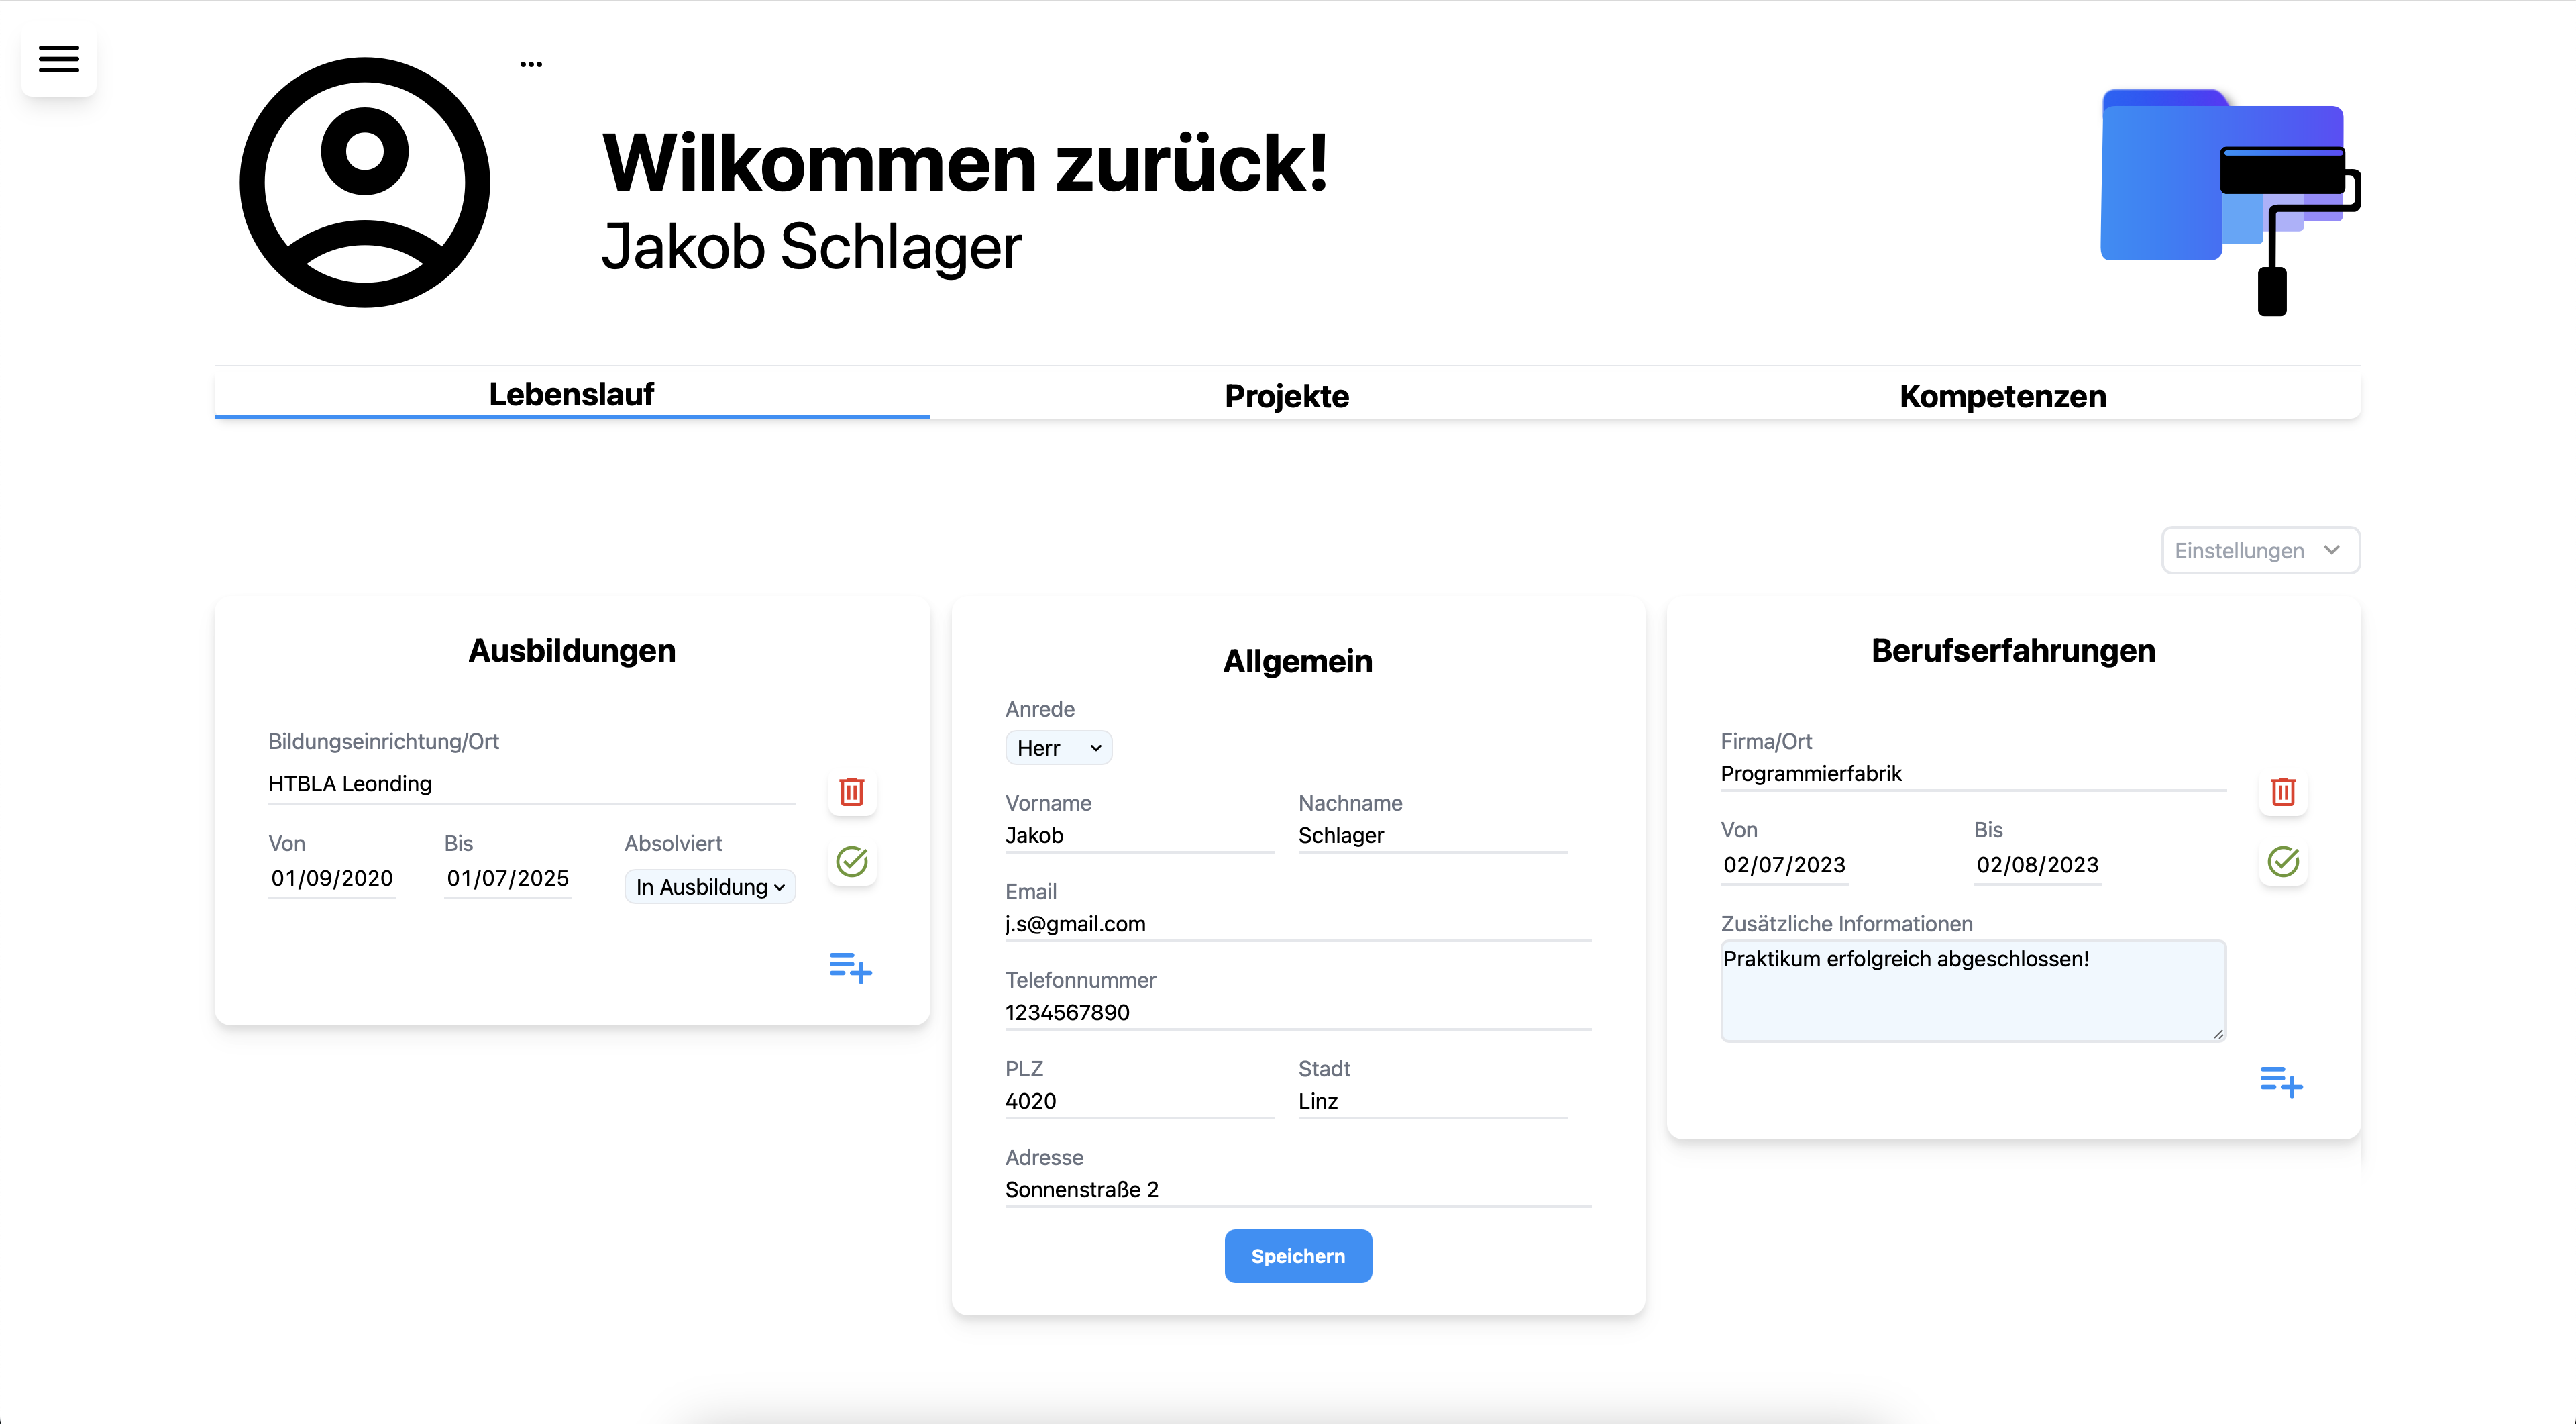
\includegraphics[width=1\linewidth]{pics//Design/Website/Startseite/Startseite_Lebenslauf.png}
    \caption{Unterseite Lebenslauf}
    \label{fig:Unterseite_Lebenslauf}
\end{figure}


\subsubsection{Allgemein}
Im mittleren Formular kann der Benutzer grundlegende Angaben zu seiner Person eintragen. Dazu gehören:

\begin{itemize}
    \item Anrede (z. B. Herr, Frau oder Divers)
\end{itemize}

\begin{itemize}
    \item Vorname und Nachname
\end{itemize}

\begin{itemize}
    \item E-Mail-Adresse
\end{itemize}

\begin{itemize}
    \item Telefonnummer
\end{itemize}

\begin{itemize}
    \item Postleitzahl und Stadt
\end{itemize}

\begin{itemize}
    \item Wohnadresse
\end{itemize}


Alle Felder sind frei editierbar, sodass der Benutzer jederzeit Änderungen vornehmen und seine Daten speichern kann.

\subsubsection{Ausbildungen}
Das linke Formular ermöglicht es dem Benutzer, seine bisherigen und aktuellen Bildungswege einzutragen. Hier können folgende Angaben gemacht werden:

Bildungseinrichtung / Ort: Der Name der Institution oder des Ausbildungsortes.
Zeitraum: Start- und Enddatum der Ausbildung.
Absolviert-Status: Eine Auswahloption, mit der der Benutzer angeben kann, ob die Ausbildung bereits abgeschlossen ist.
Ein wesentliches Feature ist die Möglichkeit, zusätzliche Ausbildungsstationen über eine Schaltfläche hinzuzufügen. Ebenso kann eine eingetragene Ausbildung bei Bedarf wieder gelöscht werden.

\subsubsection{Berufserfahrungen}

Auf der rechten Seite befindet sich das Formular für die beruflichen Erfahrungen. Hier kann der Benutzer Informationen zu bisherigen Tätigkeiten, Praktika oder anderen relevanten Erfahrungen eingeben. Die Felder umfassen:

Firma / Ort: Name des Unternehmens oder der Organisation.
Zeitraum: Start- und Enddatum der Tätigkeit.
Zusätzliche Informationen: Ein Textfeld für weitere Details, z. B. Aufgabenbereiche oder besondere Leistungen.
Auch hier gibt es die Möglichkeit, weitere Berufserfahrungen über eine Schaltfläche hinzuzufügen oder bestehende Einträge wieder zu entfernen.

\subsubsection{Benutzerfreundlichkeit und Anpassungsmöglichkeiten}
Die Unterseite „Lebenslauf“ wurde mit besonderem Fokus auf eine einfache Handhabung gestaltet. Die klar strukturierten Formulare ermöglichen eine schnelle und intuitive Dateneingabe. Die Benutzer können Einträge jederzeit bearbeiten, hinzufügen oder entfernen, was eine hohe Flexibilität gewährleistet.

Durch die klare optische Trennung der Abschnitte und die Verwendung interaktiver Elemente wie Drop-down-Menüs und Schaltflächen bietet die Unterseite eine benutzerfreundliche und übersichtliche Verwaltung der eigenen beruflichen und akademischen Laufbahn.


\subsubsection{Die Drag and Drop Funktion}


\begin{figure}[H]
    \centering
    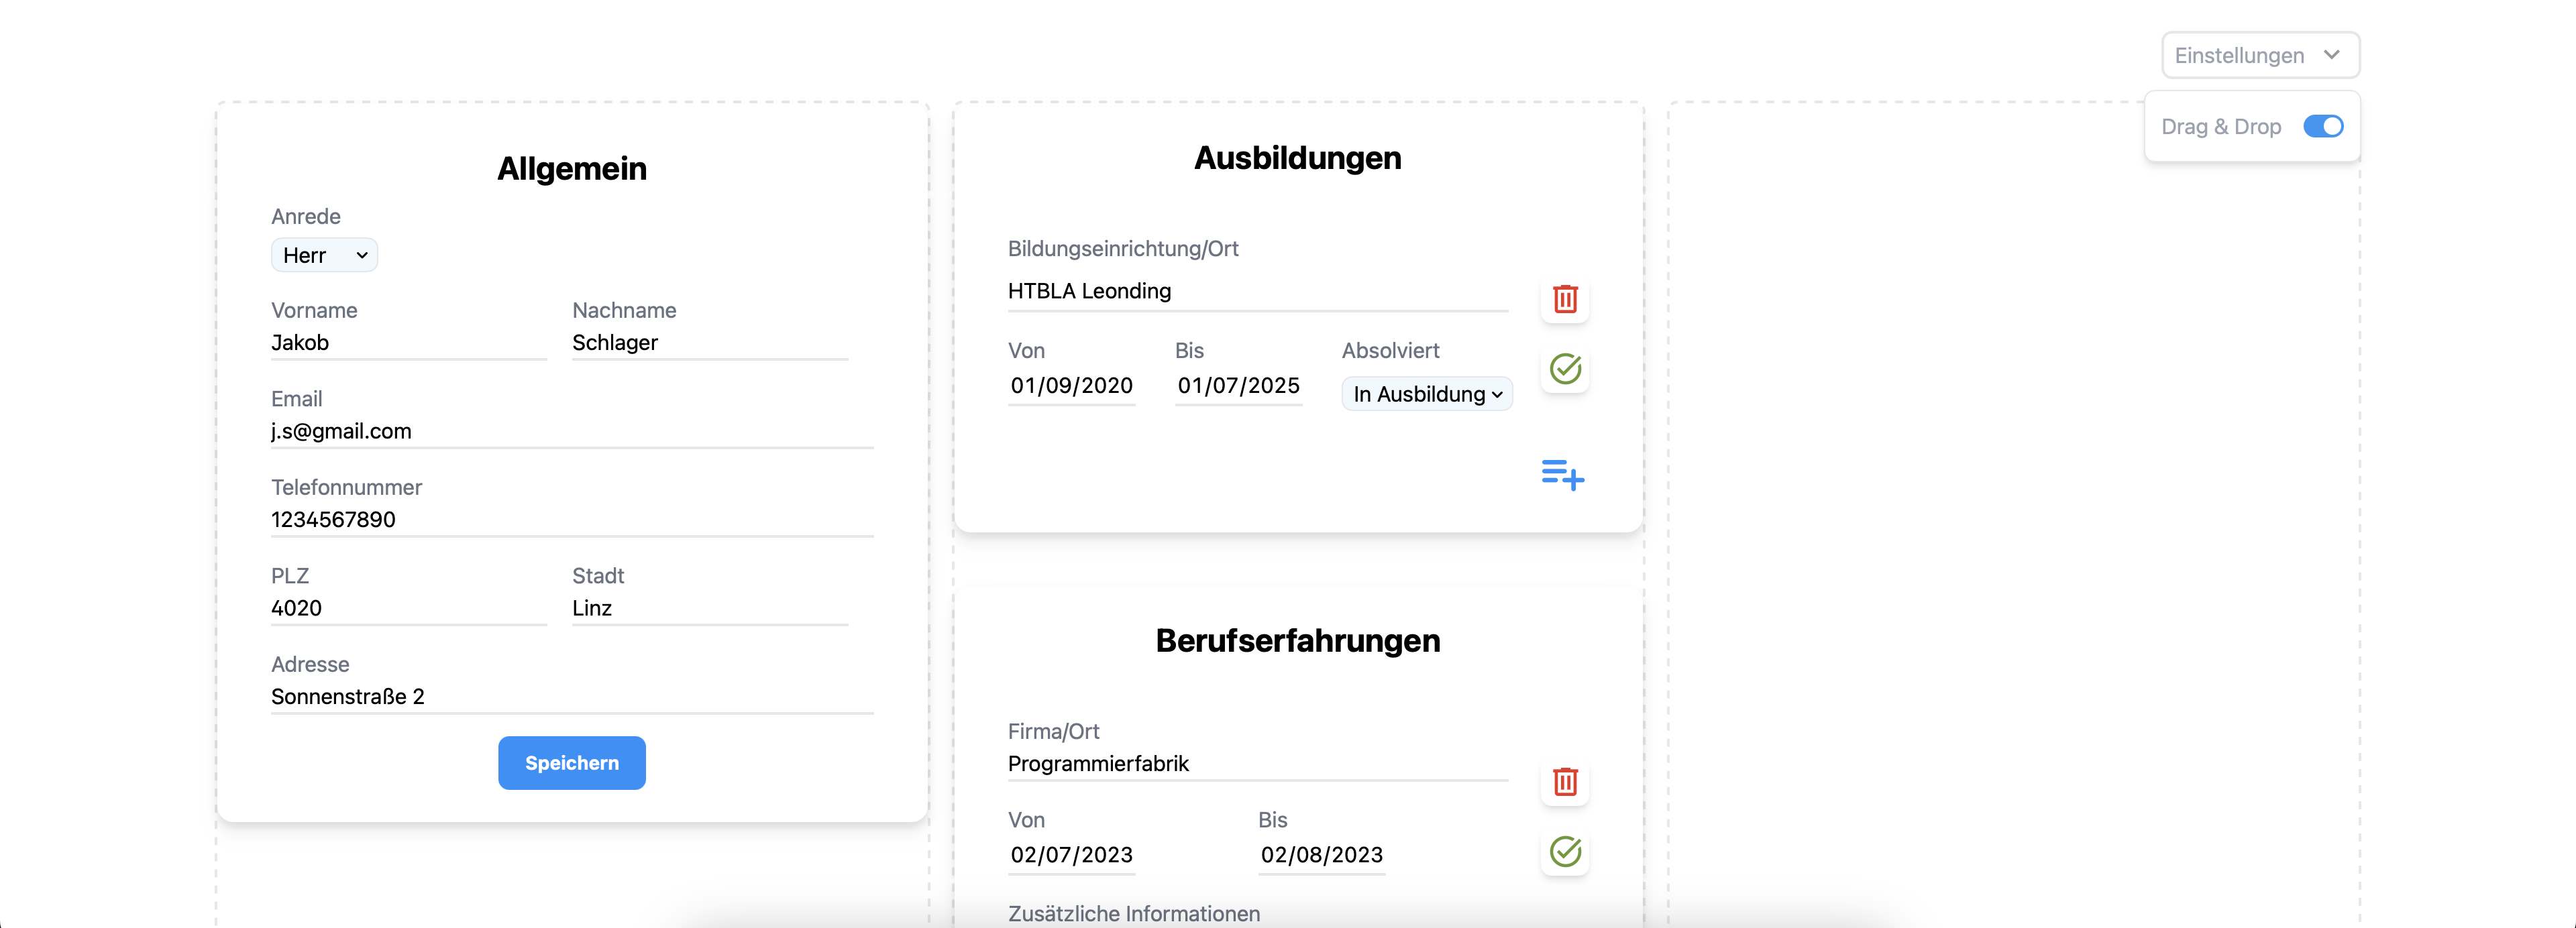
\includegraphics[width=1\linewidth]{pics//Design/Website/Startseite/D&D_showcase.png}
    \caption{Unterseite Lebenslauf}
    \label{fig:Unterseite_Lebenslauf}
\end{figure}

Ein zentrales Merkmal der Website ist die Implementierung einer Drag-and-Drop-Funktion, welche es dem Benutzer ermöglicht, die Anordnung spezifischer Elemente nach individuellen Präferenzen zu gestalten. Diese Funktion ist nicht nur auf der "Lebenslauf"-Unterseite, sondern auch bei den "Projekten" (Kunstwerken) sowie den "Kompetenzen" verfügbar.Ein besonderes Augenmerk wurde auf die Gewährleistung der Anpassungsfreiheit der Benutzeroberfläche gelegt, um den individuellen Bedürfnissen der Benutzer gerecht zu werden.

Die Aktivierung der Drag-and-Drop-Funktion erfolgt über ein Dropdown-Menü. Bei Aktivierung werden gestrichelte Hilfslinien um die verschiebbaren Elemente angezeigt, die die möglichen Positionen deutlich markieren. Gleichzeitig wird der Mauszeiger entsprechend angepasst, um anzuzeigen, dass die Formulare oder Elemente nun angeklickt und bewegt werden können.

Die visuelle Unterstützung erleichtert es dem Benutzer, die Anpassungsmöglichkeiten intuitiv zu erfassen und zu bedienen, ohne dass eine komplizierte Bedienung erforderlich ist. Die Drag-and-Drop-Funktion ermöglicht eine hohe Flexibilität und ein individuelles Nutzererlebnis, sei es beim Arrangieren von Lebenslauf-Abschnitten, der Neuanordnung von Kunstwerken oder der Strukturierung von Kompetenzen.



\subsubsection{Projekte}


\subsubsection{Kompetenzen}


\subsection{Die Gruppen-Seite}

\begin{figure}[H]
    \centering
    
\includegraphics[width=1\linewidth]{pics//Design/Website/Gruppen/Gruppen_Landing.png}
    \caption{Landing Page der Gruppenseite}
    \label{fig:Gruppen Seite}
\end{figure}

Die Gruppen-Landing-Page von Melius zeichnet sich durch eine intuitive und moderne Benutzererfahrung aus, die den Community-Gedanken der Plattform unterstreicht. Sie ermöglicht es Nutzern, neue Gruppen effizient zu erstellen oder bestehenden Gruppen beizutreten. Hinsichtlich des Designs und der Struktur ist festzustellen, dass die linke Seite der Seite den Nutzer mit der klaren Botschaft "Willkommen bei Gruppen" begrüßt. Darunter befindet sich eine Suchleiste, mit der Nutzer gezielt nach Gruppen suchen können. Diese Funktion erleichtert den Einstieg und ermöglicht eine direkte Navigation. 

Darunter befinden sich zwei zentrale \textbf{Call-to-Action-Buttons:}

\begin{itemize}
    \item Der blaue Button mit der Beschriftung "Eine eigene Gruppe erstellen" ermöglicht den schnellen Aufbau einer neuen Gruppe innerhalb der Plattform.
\end{itemize}

\begin{itemize}
    \item Der lila Button mit der Beschriftung "Meine Gruppen" führt den Nutzer zu seinen bereits erstellten oder beigetretenen Gruppen.
\end{itemize}

Die visuelle Gestaltung der Plattform ist auf eine harmonische Ästhetik ausgerichtet, die eine visuelle Wiedererkennung ermöglicht. Auf der rechten Seite der Startseite befindet sich ein großes, stilisiertes Gruppen-Icon, das die Idee der Vernetzung symbolisiert. Der Hintergrund ist mit diagonalen Farbverläufen in Blau- und Lilatönen gestaltet, die sich an den Primärfarben der Applikation orientieren.

Die Seite ist übersichtlich gestaltet, sodass sich Nutzer intuitiv zurechtfinden. Dies ist ein Aspekt der Funktionalität. Die zentral platzierten Buttons ermöglichen eine schnelle und unkomplizierte Nutzung der Gruppenfunktionen.

Die Integration einer \textbf{Suchleiste} erleichtert es den Nutzern, gezielt nach bestehenden Gruppen zu suchen.


\subsubsection{Suchleiste}

\begin{figure}[H]
    \centering
    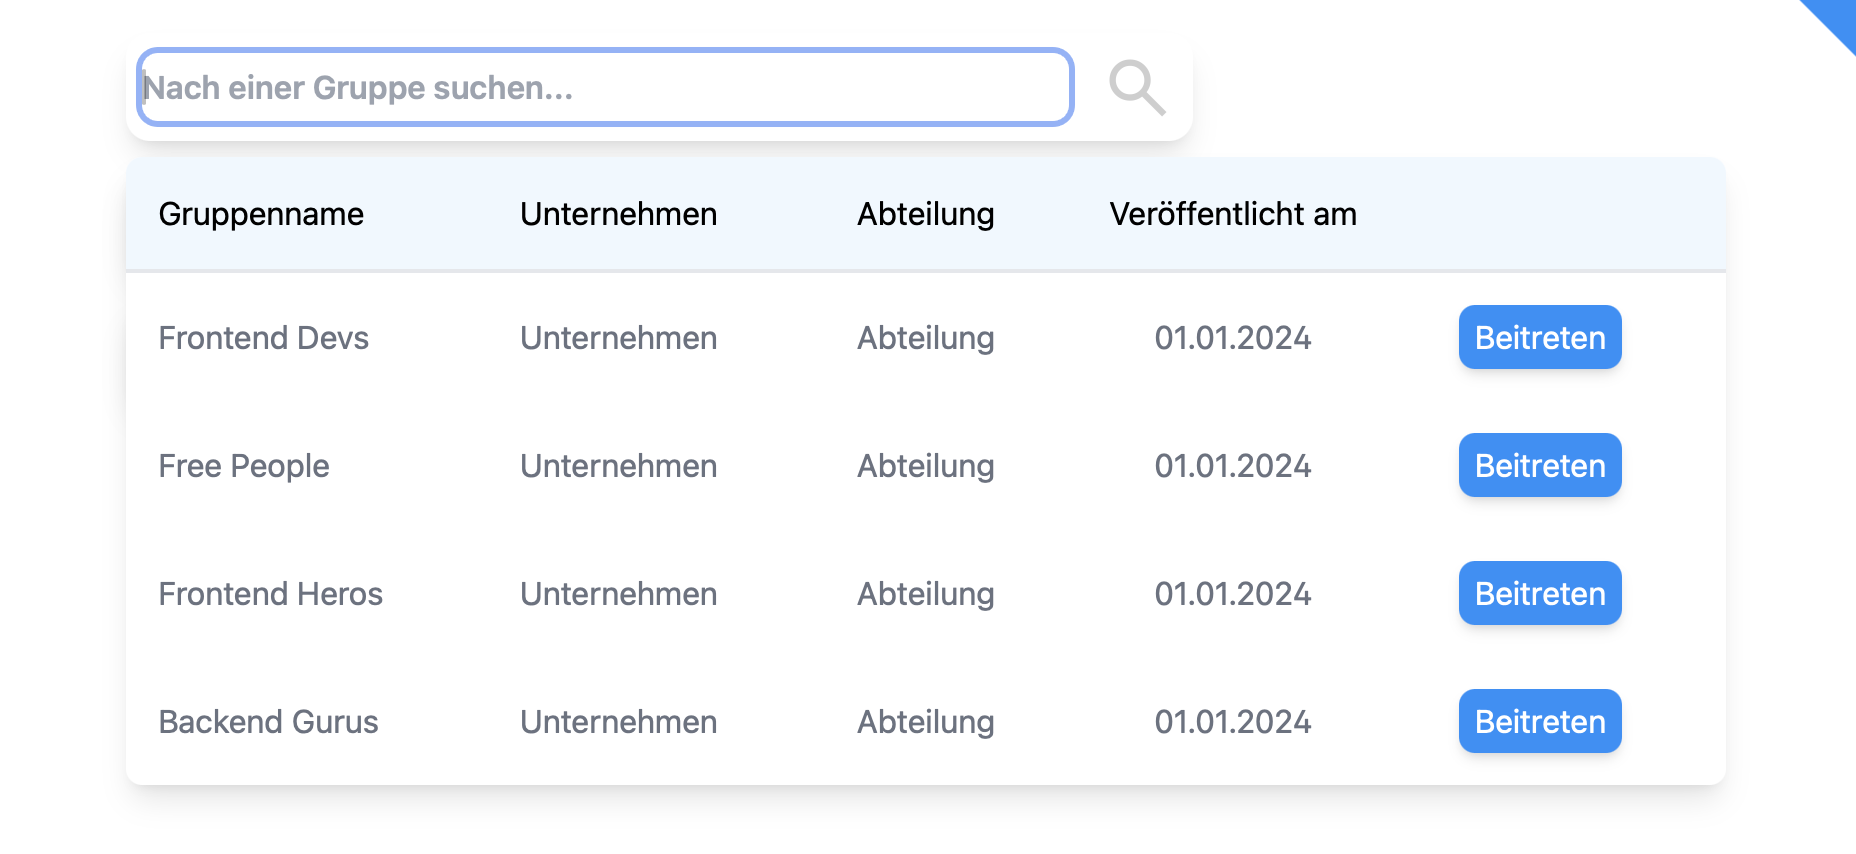
\includegraphics[width=0.75\linewidth]{pics//Design/Website/Gruppen/Suchergebnisse.png}
    \caption{Suchergebnisse}
    \label{fig:Suchergebnisse}
\end{figure}

Die Suchfunktion ermöglicht es den Nutzern, gezielt nach Gruppen zu suchen. Beim Eintippen eines Gruppennamens filtert das System automatisch die verfügbaren Gruppen und zeigt passende Ergebnisse an. Sollte keine Gruppe mit dem eingegebenen Namen existieren, wird eine entsprechende Meldung angezeigt.
Die Ergebnisliste besteht aus einer Tabelle mit folgenden Spalten:

\begin{itemize}
    \item der Gruppenname
\end{itemize}

\begin{itemize}
    \item das dazugehörige Unternehmen
\end{itemize}

\begin{itemize}
    \item die spezifische Abteilung innerhalb des Unternehmens
\end{itemize}

\begin{itemize}
    \item das Erstellungsdatum der Gruppe
\end{itemize}
In der Nähe jeder Gruppe befindet sich ein blauer Button mit der Beschriftung "Beitreten". Dieser führt den Benutzer zur nächsten Ansicht, in der ein Beitritt zur Gruppe möglich ist.


\begin{figure}[H]
    \centering
    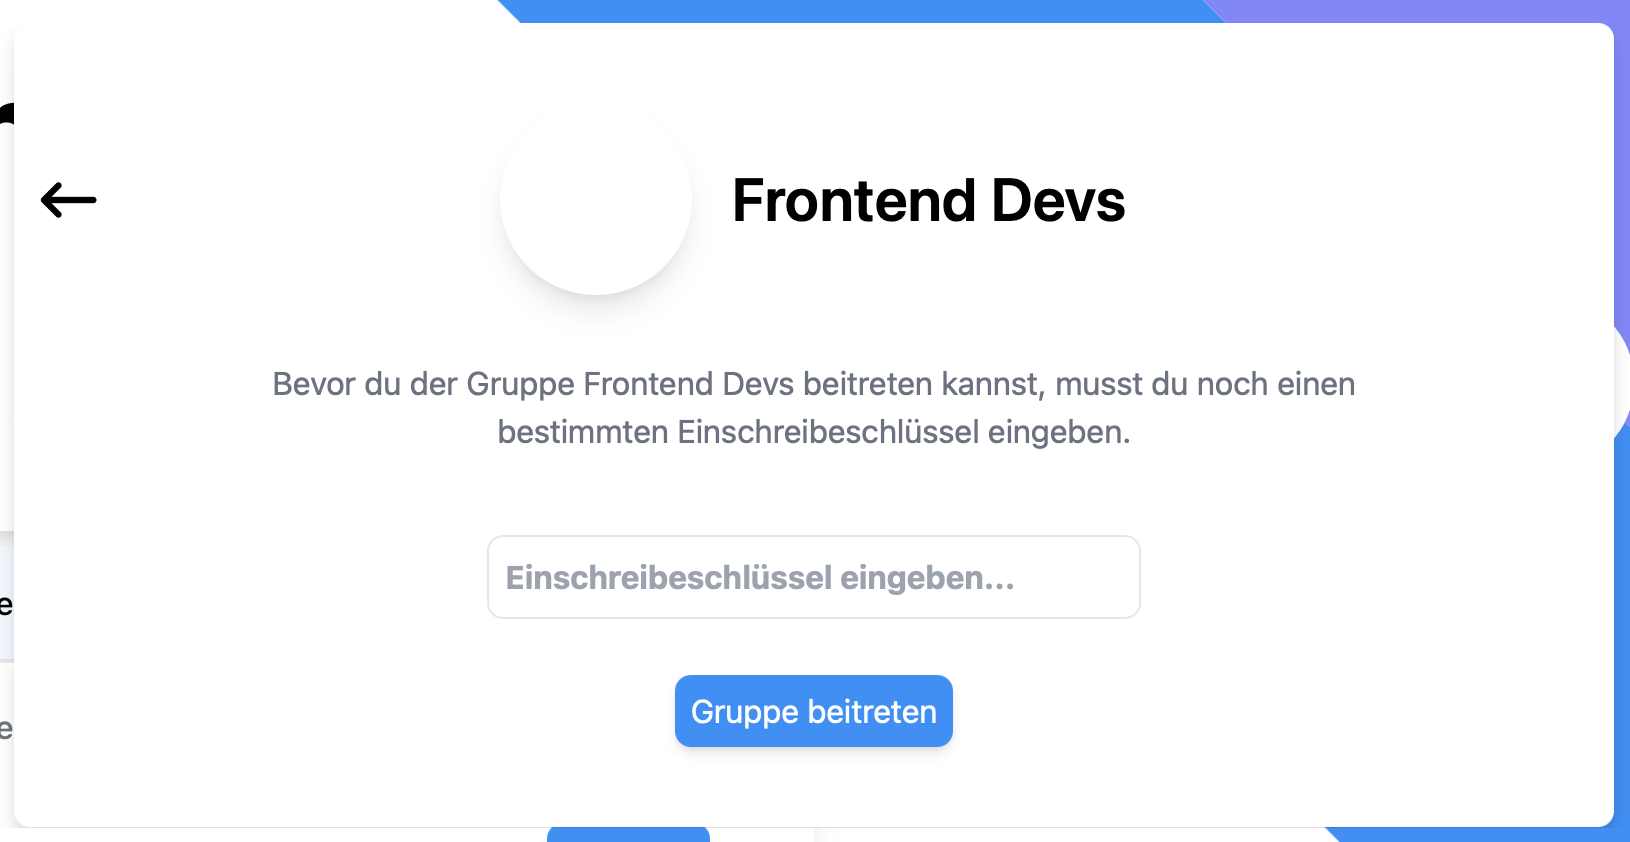
\includegraphics[width=0.75\linewidth]{pics//Design/Website/Gruppen/GroupForm_Login.png}
    \caption{Eingabeformular zum beitreten einer Gruppe}
    \label{fig:Eingabeformular}
\end{figure}

Sobald der Nutzer eine Gruppe ausgewählt hat, wird er zur Beitrittsansicht weitergeleitet. Hier wird er aufgefordert, einen Einschreibeschlüssel einzugeben, um der Gruppe beizutreten.

Diese Sicherheitsmaßnahme stellt sicher, dass nur autorisierte Personen Zugang zu bestimmten Gruppen erhalten. Dies kann besonders in geschlossenen Unternehmensgruppen oder spezifischen Fachgruppen wichtig sein, um eine kontrollierte Mitgliederstruktur zu gewährleisten.

Das Design dieser Ansicht ist minimalistisch und auf eine klare Benutzerführung ausgerichtet:

\begin{itemize}
    \item Der Gruppenname wird prominent in großer, fetter Schrift dargestellt, sodass der Nutzer eindeutig erkennen kann, welcher Gruppe er beitreten möchte.
\end{itemize}

\begin{itemize}
    \item Direkt darunter befindet sich eine kurze Erklärung, die dem Nutzer mitteilt, dass ein Einschreibeschlüssel erforderlich ist. Diese Anleitung hilft, Verwirrung zu vermeiden und macht deutlich, dass ohne den Schlüssel kein Beitritt möglich ist.
\end{itemize}

\begin{itemize}
    \item Ein Eingabefeld erlaubt es dem Nutzer, den Einschreibeschlüssel einzugeben. Das Feld ist dezent gestaltet und vermittelt durch den Platzhaltertext "Einschreibeschlüssel eingeben..." eine klare Anweisung.
\end{itemize}

\begin{itemize}
    \item Der "Gruppe beitreten"-Button hebt sich durch seine kräftige blaue Farbe deutlich von der restlichen Oberfläche ab. Sobald der Nutzer den Schlüssel eingegeben hat, kann er diesen Button klicken, um der Gruppe beizutreten.
\end{itemize}

Falls der Einschreibeschlüssel korrekt ist, wird der Nutzer erfolgreich zur Gruppe hinzugefügt und erhält Zugriff auf deren Inhalte und Mitglieder. Sollte der Schlüssel falsch sein, kann das System eine Fehlermeldung ausgeben, um den Nutzer darauf hinzuweisen.

Diese Beitrittsfunktion stellt sicher dsn ans d, dass Gruppen geschützt bleiben, während gleichzeitig eine einfache Möglichkeit besteht, neue Mitglieder aufzunehmen.


\subsubsection{Gruppen erstellen}

\subsubsection{Meine Gruppen}

\subsection{Die Einstellungen}

